\chapter{Experimentación y Resultados}

\section{Medidas y Métricas Utilizadas}
Para evaluar la aptitud funcional de las bandas seleccionadas, la métrica elegida fue el F1-Score. Esta medida es fundamental porque balancea la precisión y la sensibilidad, penalizando rigurosamente los falsos negativos (clasificar un higo infectado como sano), un escenario que representa un riesgo inaceptable para la seguridad alimentaria \cite{cruz-carrasco_detection_2024}.
\begin{equation}
    F1=2 \times{\frac{Precision\times{Recall}}{Precision+Recall}}
\end{equation}

\section{Configuraciones Experimentales}
Ambos algoritmos metaheurísticos fueron ejecutados de manera independiente 30 veces para cada tamaño de subconjunto objetivo ($k \in \{3, 5, 6\}$) \cite{eiben_introduction_2015}. En las siguientes tablas se muestran las configuraciones del GA, PSO y SVM respectivamente:

\begin{table}[H] 
%\small % Change table font size
\caption{Parametros del Algoritmo Genético.\label{tab:ga_params}}
%\isPreprints{\centering}{} % Only used for preprints
\begin{tabularx}{\textwidth}{CCCCC}
\toprule
\textbf{Generaciones} & \textbf{Tamaño de población} & \textbf{Tipo de selección} & \textbf{Cruza} & \textbf{Tasa de mutación}\\
\midrule
350 & 250 & Torndeo de 2 & Cruza de un punto & 2.5\\
\bottomrule
\end{tabularx}
\noindent
\end{table}

\begin{table}[H] 
%\small % Change table font size
\caption{Parametros de PSO.\label{tab:pso_params}}
%\isPreprints{\centering}{} % Only used for preprints
\begin{tabularx}{\textwidth}{CCCCCC}
\toprule
\textbf{Iteraciones} & \textbf{Particulas} & \textbf{Coeficiente cognitivo (C1)} & \textbf{Coeficiente social (C2)} & \textbf{Inercia} & \textbf{Tasa de mutación}\\
\midrule
650 & 200 & 0.4 a 2.5 & 2.5 a 0.4 & 0.7 & 0.2\\
\bottomrule
\end{tabularx}
\noindent
\end{table}

\begin{table}[H] 
%\small % Change table font size
\caption{Parametros de SVM.\label{tab:svm_params}}
%\isPreprints{\centering}{} % Only used for preprints
\begin{tabularx}{\textwidth}{CCCCC}
\toprule
\textbf{Implementación} & \textbf{Kernel} & \textbf{regularización ($C$)} & \textbf{Gamma ($\gamma$)} & \textbf{Método de validación}\\
\midrule
Fast evaluator       & RBF & Fixed 1.0             & Fixed scale & k-fold CV ($k=3$)\\ \\
Exhaustive evaluator & RBF & Grid search 0.1 a 1000 & Grid search 0.001 a 1 & k-fold CV ($k=5$)\\
\bottomrule
\end{tabularx}
\noindent
\end{table}

\section{Caracterización Espectral de las Muestras}
Como paso previo a la evaluación del rendimiento de los algoritmos de clasificación y optimización, se realizó un análisis exploratorio del comportamiento espectral de las muestras en el rango VNIR (400 nm a 1000 nm). Este análisis es fundamental para comprender la naturaleza de los datos y justificar la pertinencia de las características extraídas.

La Figura \ref{fig:mean_std_reflectance} ilustra las firmas espectrales promedio de reflectancia tanto para la clase de frutos sanos (control) como para la clase con infección severa por Aspergillus flavus. Las regiones sombreadas representan la desviación estándar, ilustrando la dispersión de los datos dentro de cada clase. Como se puede observar, los patrones espectrales de ambas clases presentan una similitud visual extremadamente alta, evidenciando un solapamiento casi total en la región del espectro visible (400 - 700 nm). Se aprecia una divergencia sutil en la intensidad de reflectancia únicamente en la región del infrarrojo cercano (NIR, 700 - 1000 nm), un fenómeno atribuible a la degradación de la estructura celular interna del tejido del higo inducida por la colonización fúngica. Este alto grado de solapamiento espectral confirma la complejidad intrínseca de la tarea de clasificación y justifica la necesidad de emplear técnicas avanzadas de selección de bandas en lugar de umbrales espectrales simples.

Sin embargo, el análisis de la variabilidad espacial revela un comportamiento diametralmente distinto. La Figura 5.1b presenta la desviación estándar de la reflectancia en función de la longitud de onda para ambas clases. En esta representación, se evidencia de manera contundente que las muestras infectadas exhiben una variabilidad espacial (textural) consistentemente superior en comparación con los higos sanos a lo largo de todo el espectro.

Esta evidencia empírica respalda la hipótesis central de la metodología propuesta: la infección fúngica, altera la heterogeneidad en la superficie del higo. Por lo tanto, se confirma que la inclusión de la desviación estándar ($\sigma$) en el vector de características no es redundante, sino que aporta información discriminatoria crítica que la reflectancia media ($\mu$) por sí sola es incapaz de capturar.

\begin{figure}[H]
\centering
\subfloat[\centering]{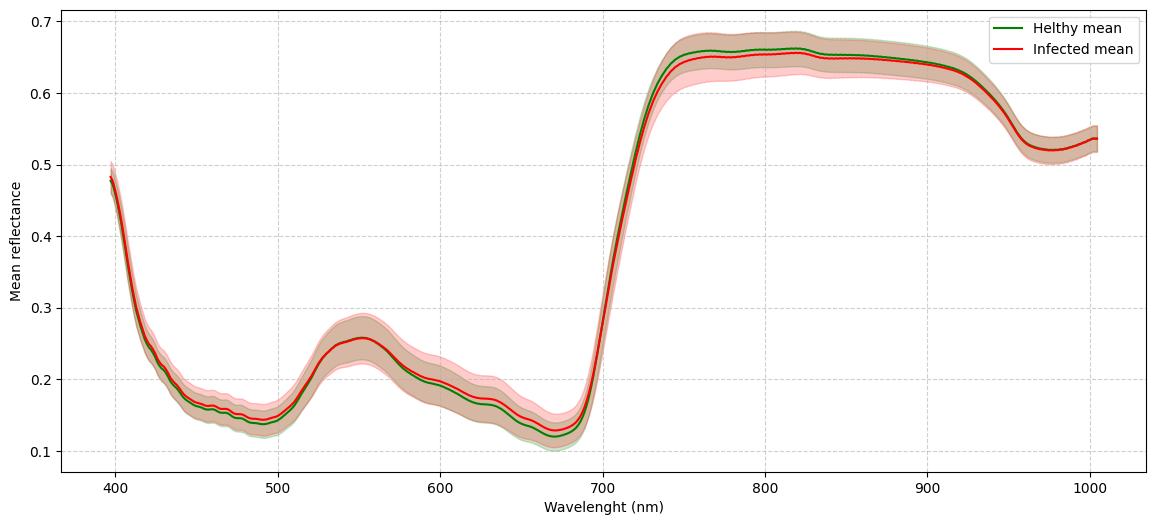
\includegraphics[width=13.0cm]{Imagenes/spectral_signature_mean_reflectance.png}}\\
\subfloat[\centering]{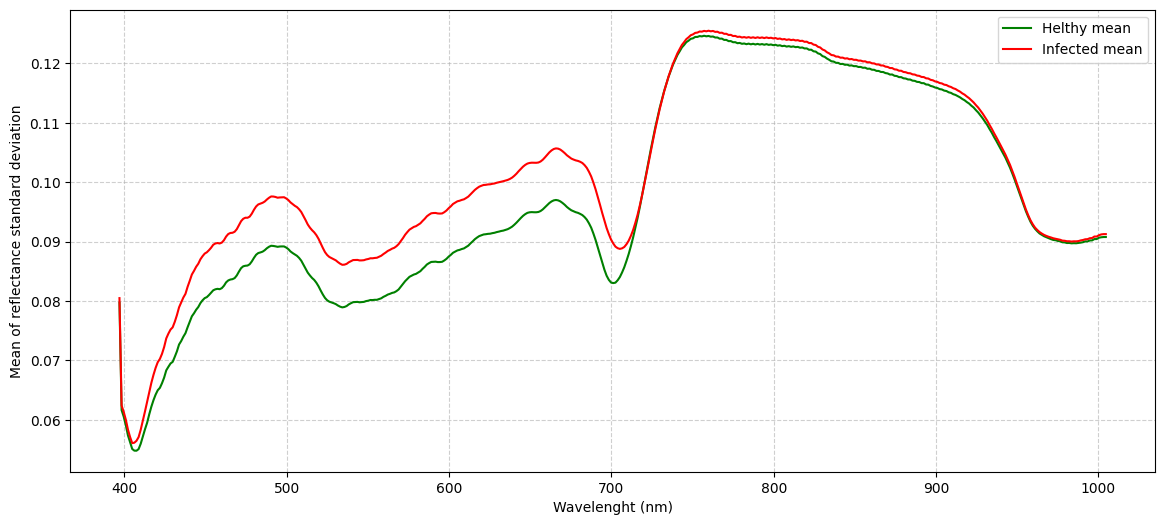
\includegraphics[width=13.0cm]{Imagenes/spectral_signature_mean_standard_deviation.png}}
\caption{Caracterización espectral de las muestras de higo. (\textbf{a}) Firmas de reflectancia media mostrando la tendencia central. (\textbf{b}) Desviación estándar de la reflectancia representando la variabilidad espacial (textura).\label{fig:mean_std_reflectance}}
\end{figure} 

\section{Resultados}
Una vez confirmada la relevancia espectral de las características extraídas, se procedió a evaluar el rendimiento cuantitativo de los algoritmos metaheurísticos en la tarea de reducción de dimensionalidad y clasificación.

\subsection{Resultados de la Construcción de Características}
El primer experimento tuvo como objetivo validar computacionalmente la hipótesis planteada en la sección anterior: la superioridad del vector de características combinado ($\mu + \sigma$) sobre el uso exclusivo de la reflectancia media ($\mu$).
Para ello, se ejecutó el proceso de selección de bandas bajo ambas configuraciones, estableciendo tamaños de subconjuntos objetivo de $k \in\{3, 5, 6\}$ a lo largo de 30 ejecuciones independientes.

Los resultados, promediados y presentados en la Tabla \ref{tab:ga_performance}, demuestran que la inclusión de la desviación estándar mejora significativamente la exactitud del modelo. Incrementando la métrica \textit{F1-Score} particularment en los subconjuntos de menor dimensionalidad, alcanzando una mejora del $+9.2\%$ para $k=3$ y del $+7.2\%$ para $k=5$
\begin{table}[H] 
%\small % Change table font size
\caption{Comparación de desempeño GA (F1-Score promedio) entre características.\label{tab:ga_performance}}
%\isPreprints{\centering}{} % Only used for preprints
\begin{tabularx}{\textwidth}{CCCC}
\toprule
\textbf{Tamaño de individuo} & \textbf{Solo media de reflectancia ($\mu$)} & \textbf{Características combinadas ($\mu + \sigma$)} & \textbf{Mejora (\%)} \\
\midrule
3 Bandas & 0.663 & 0.755 & +9.2\% \\
5 Bandas & 0.698 & 0.77  & +7.2\% \\
6 Bandas & 0.721 & 0.773 & +5.2\%  \\
\bottomrule
\end{tabularx}
\noindent
\end{table}

Adicionalmente, el análisis del historial de convergencia del Algoritmo Genético (Figura \ref{fig:ga_convergence}) confirma que la estrategia combinada no solo inicia con una aptitud superior desde las primeras generaciones, sino que mantiene una trayectoria de optimización mucho más robusta. Esto sugiere que la información textural estabiliza el espacio de búsqueda, permitiendo a la metaheurística eludir mínimos locales y converger hacia soluciones de mayor calidad con mayor eficiencia.
\begin{figure}[H]
%\begin{adjustwidth}{-\extralength}{0cm}
\centering
\subfloat[\centering]{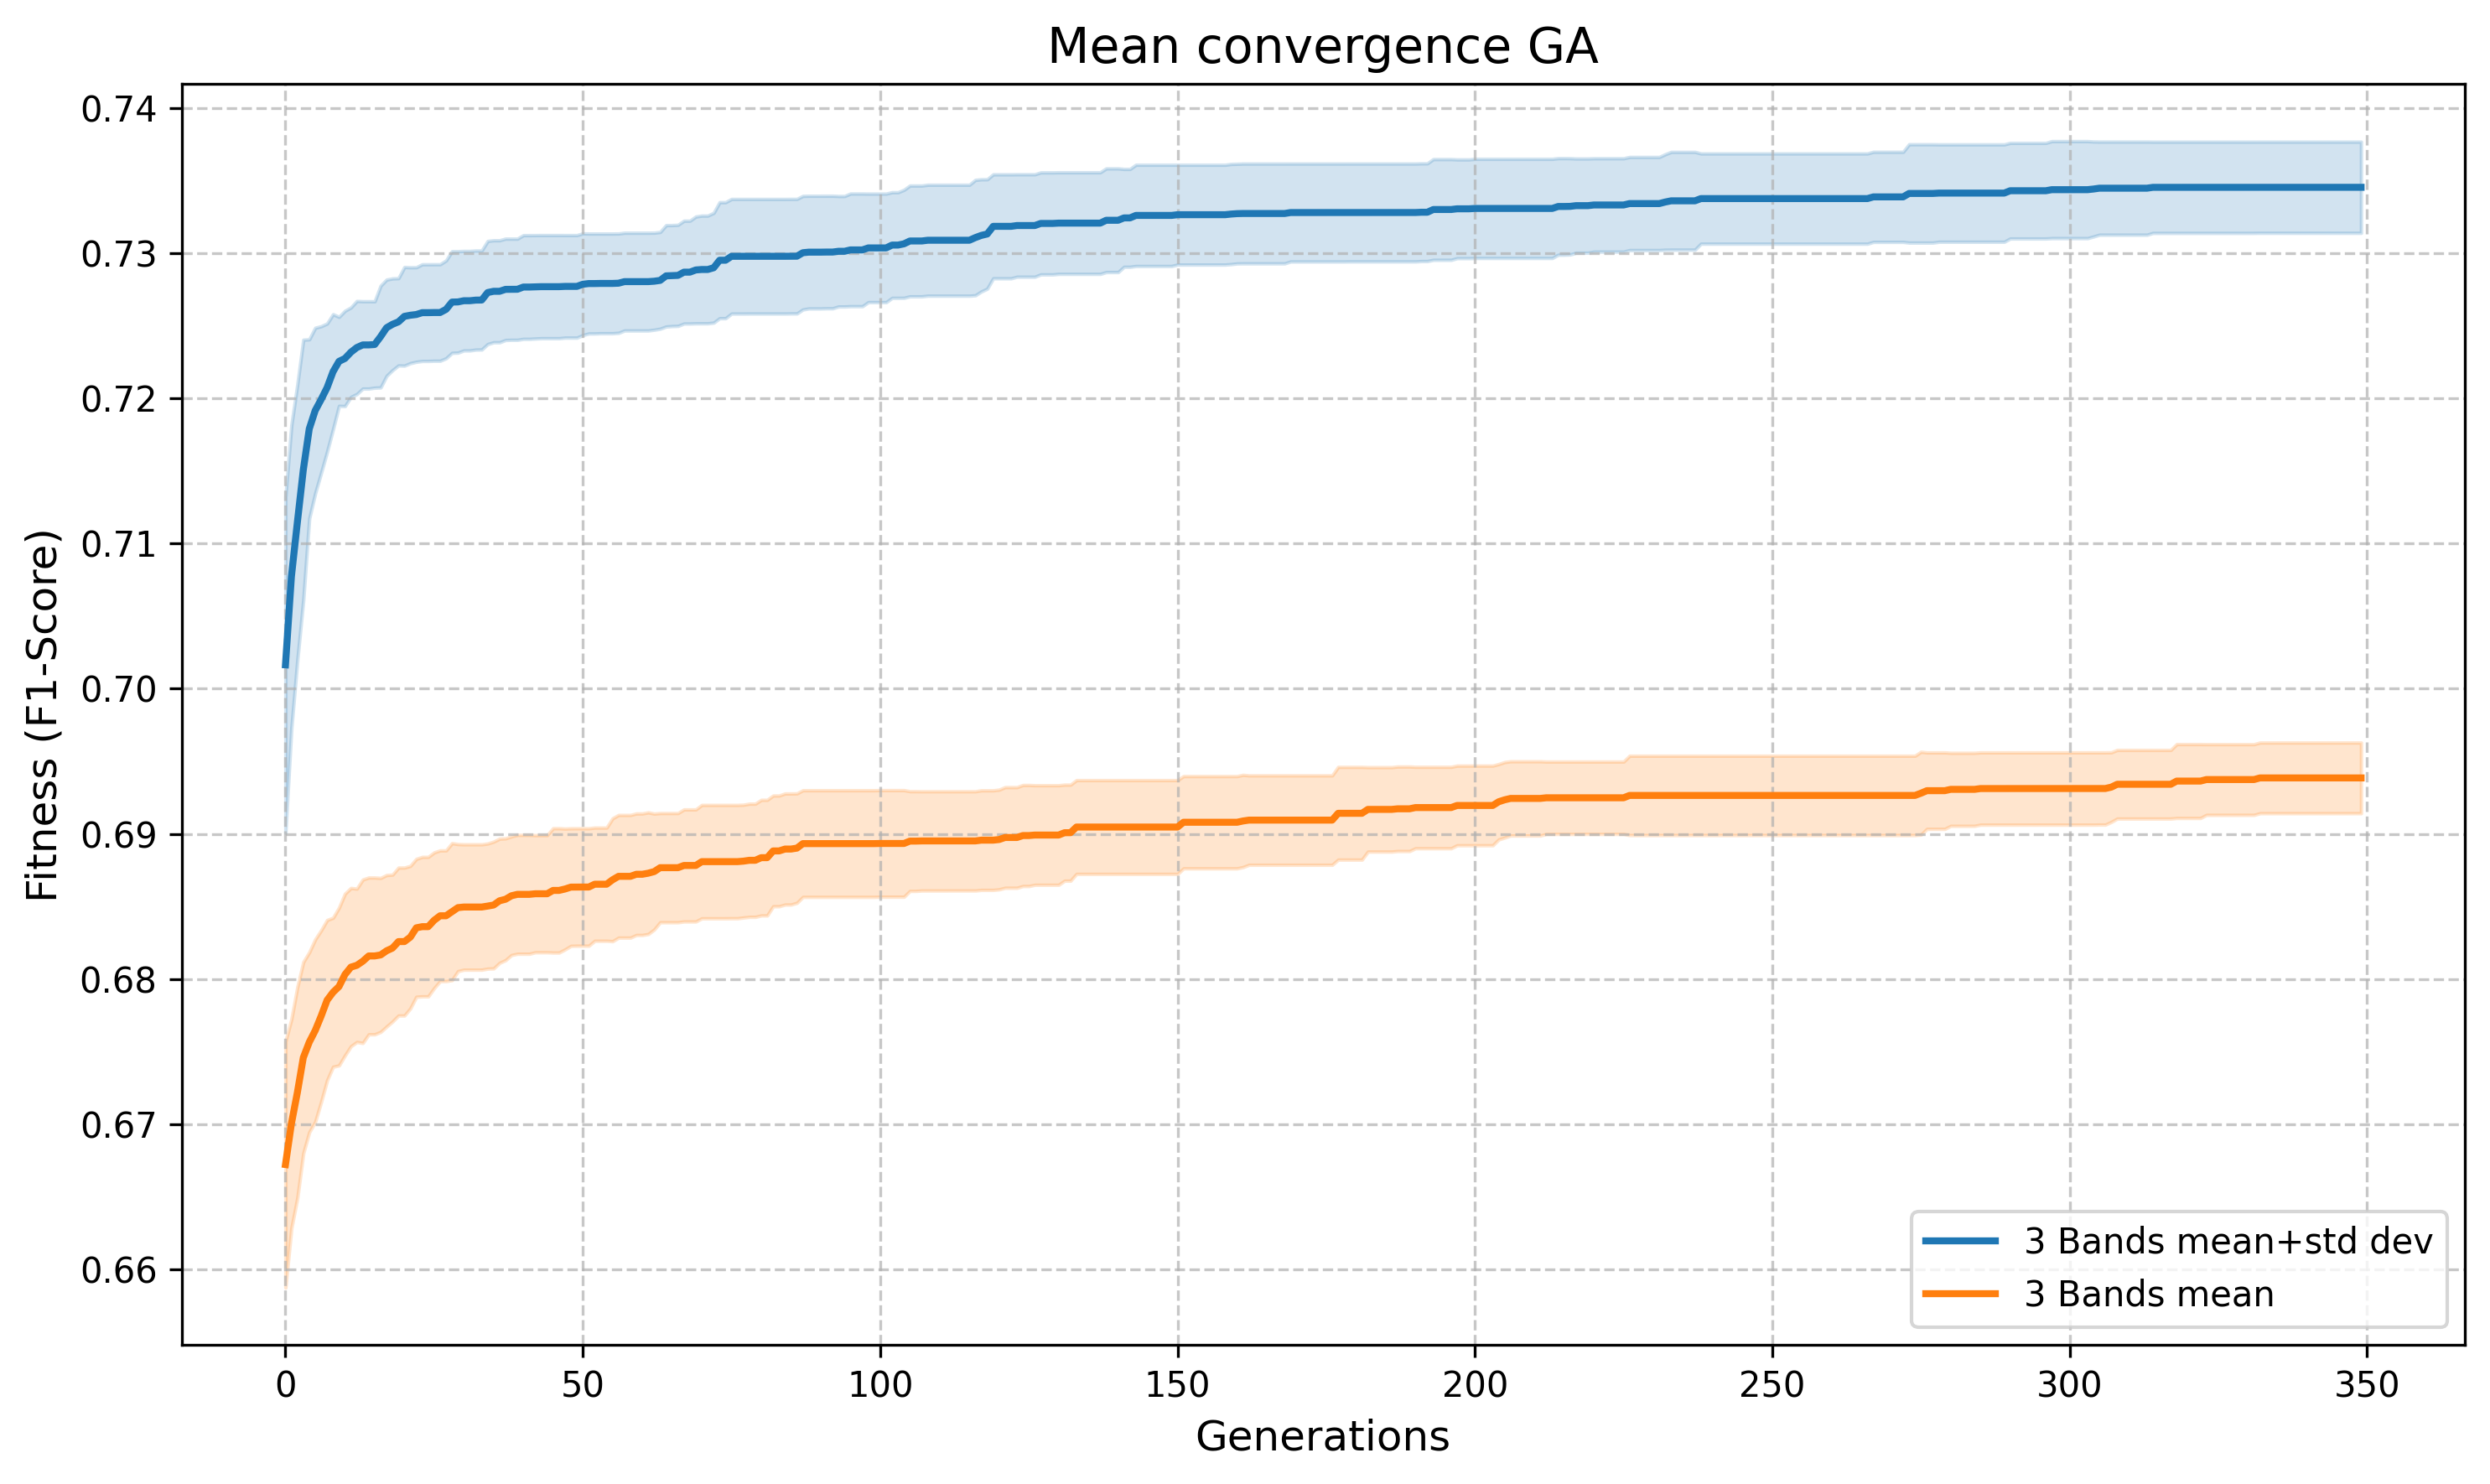
\includegraphics[width=8.2cm]{Imagenes/mean_convergence_3b.png}} 
%\hfill
\subfloat[\centering]{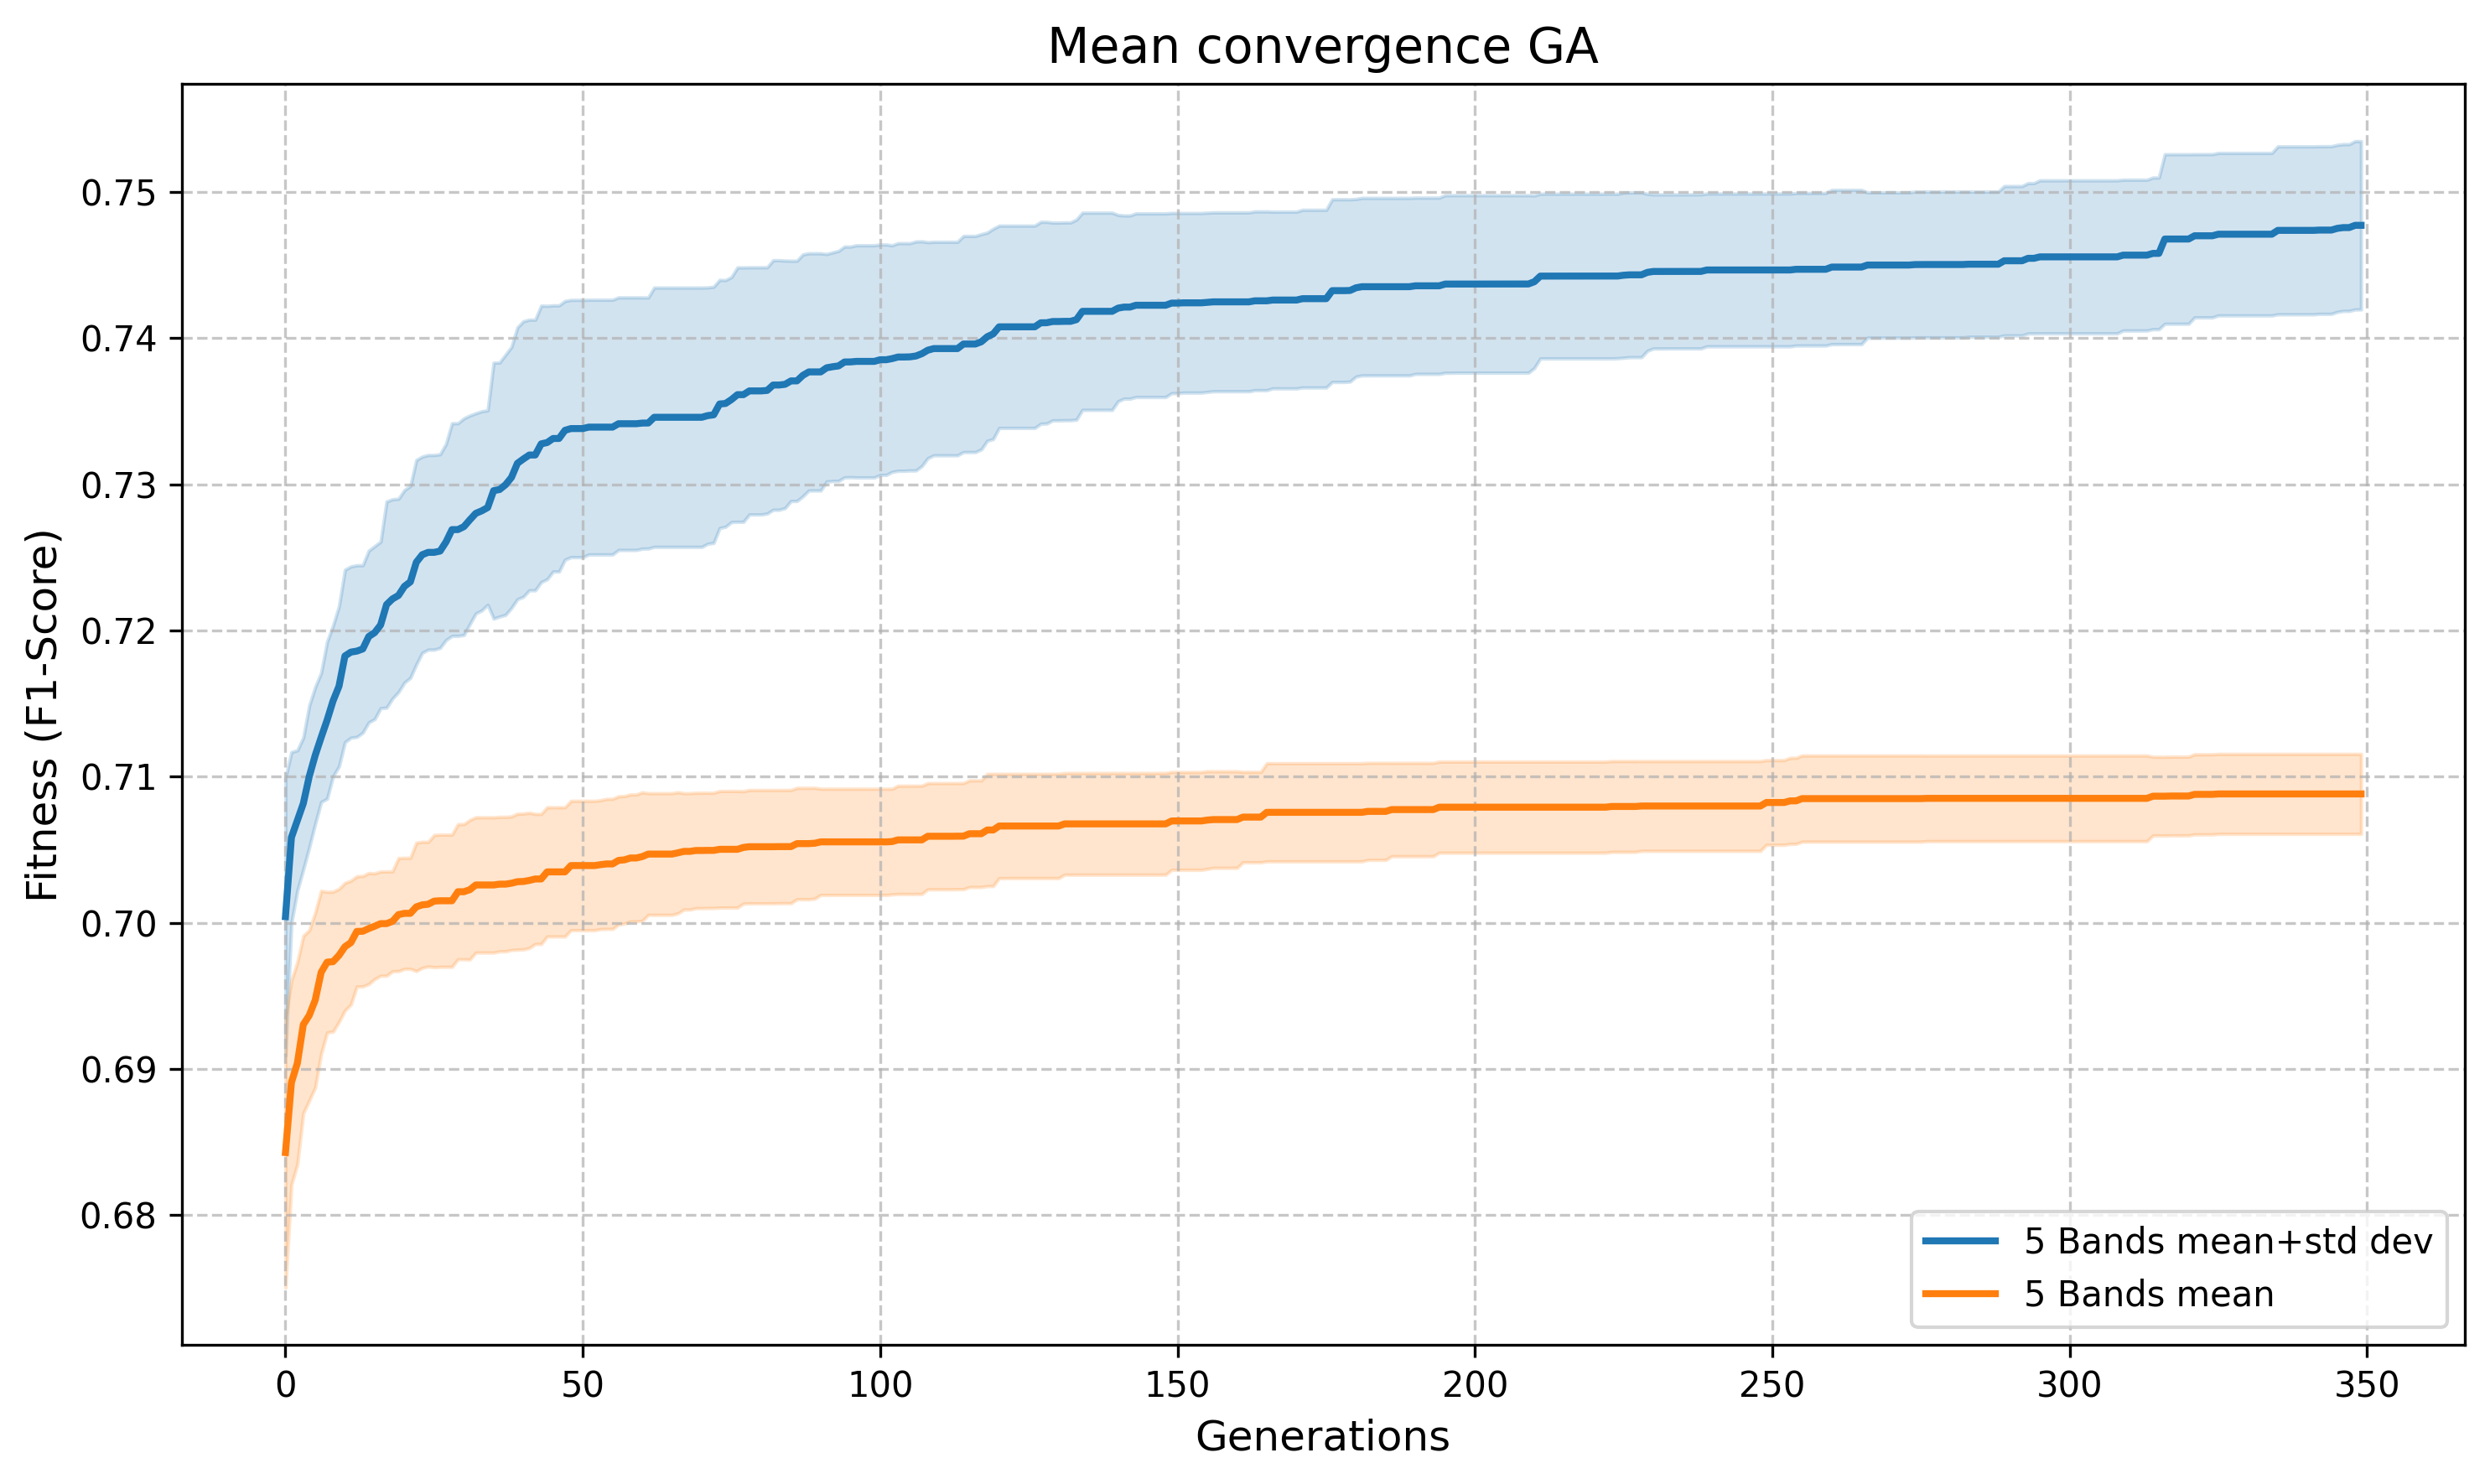
\includegraphics[width=8.2cm]{Imagenes/mean_convergence_5b.png}}\\
\subfloat[\centering]{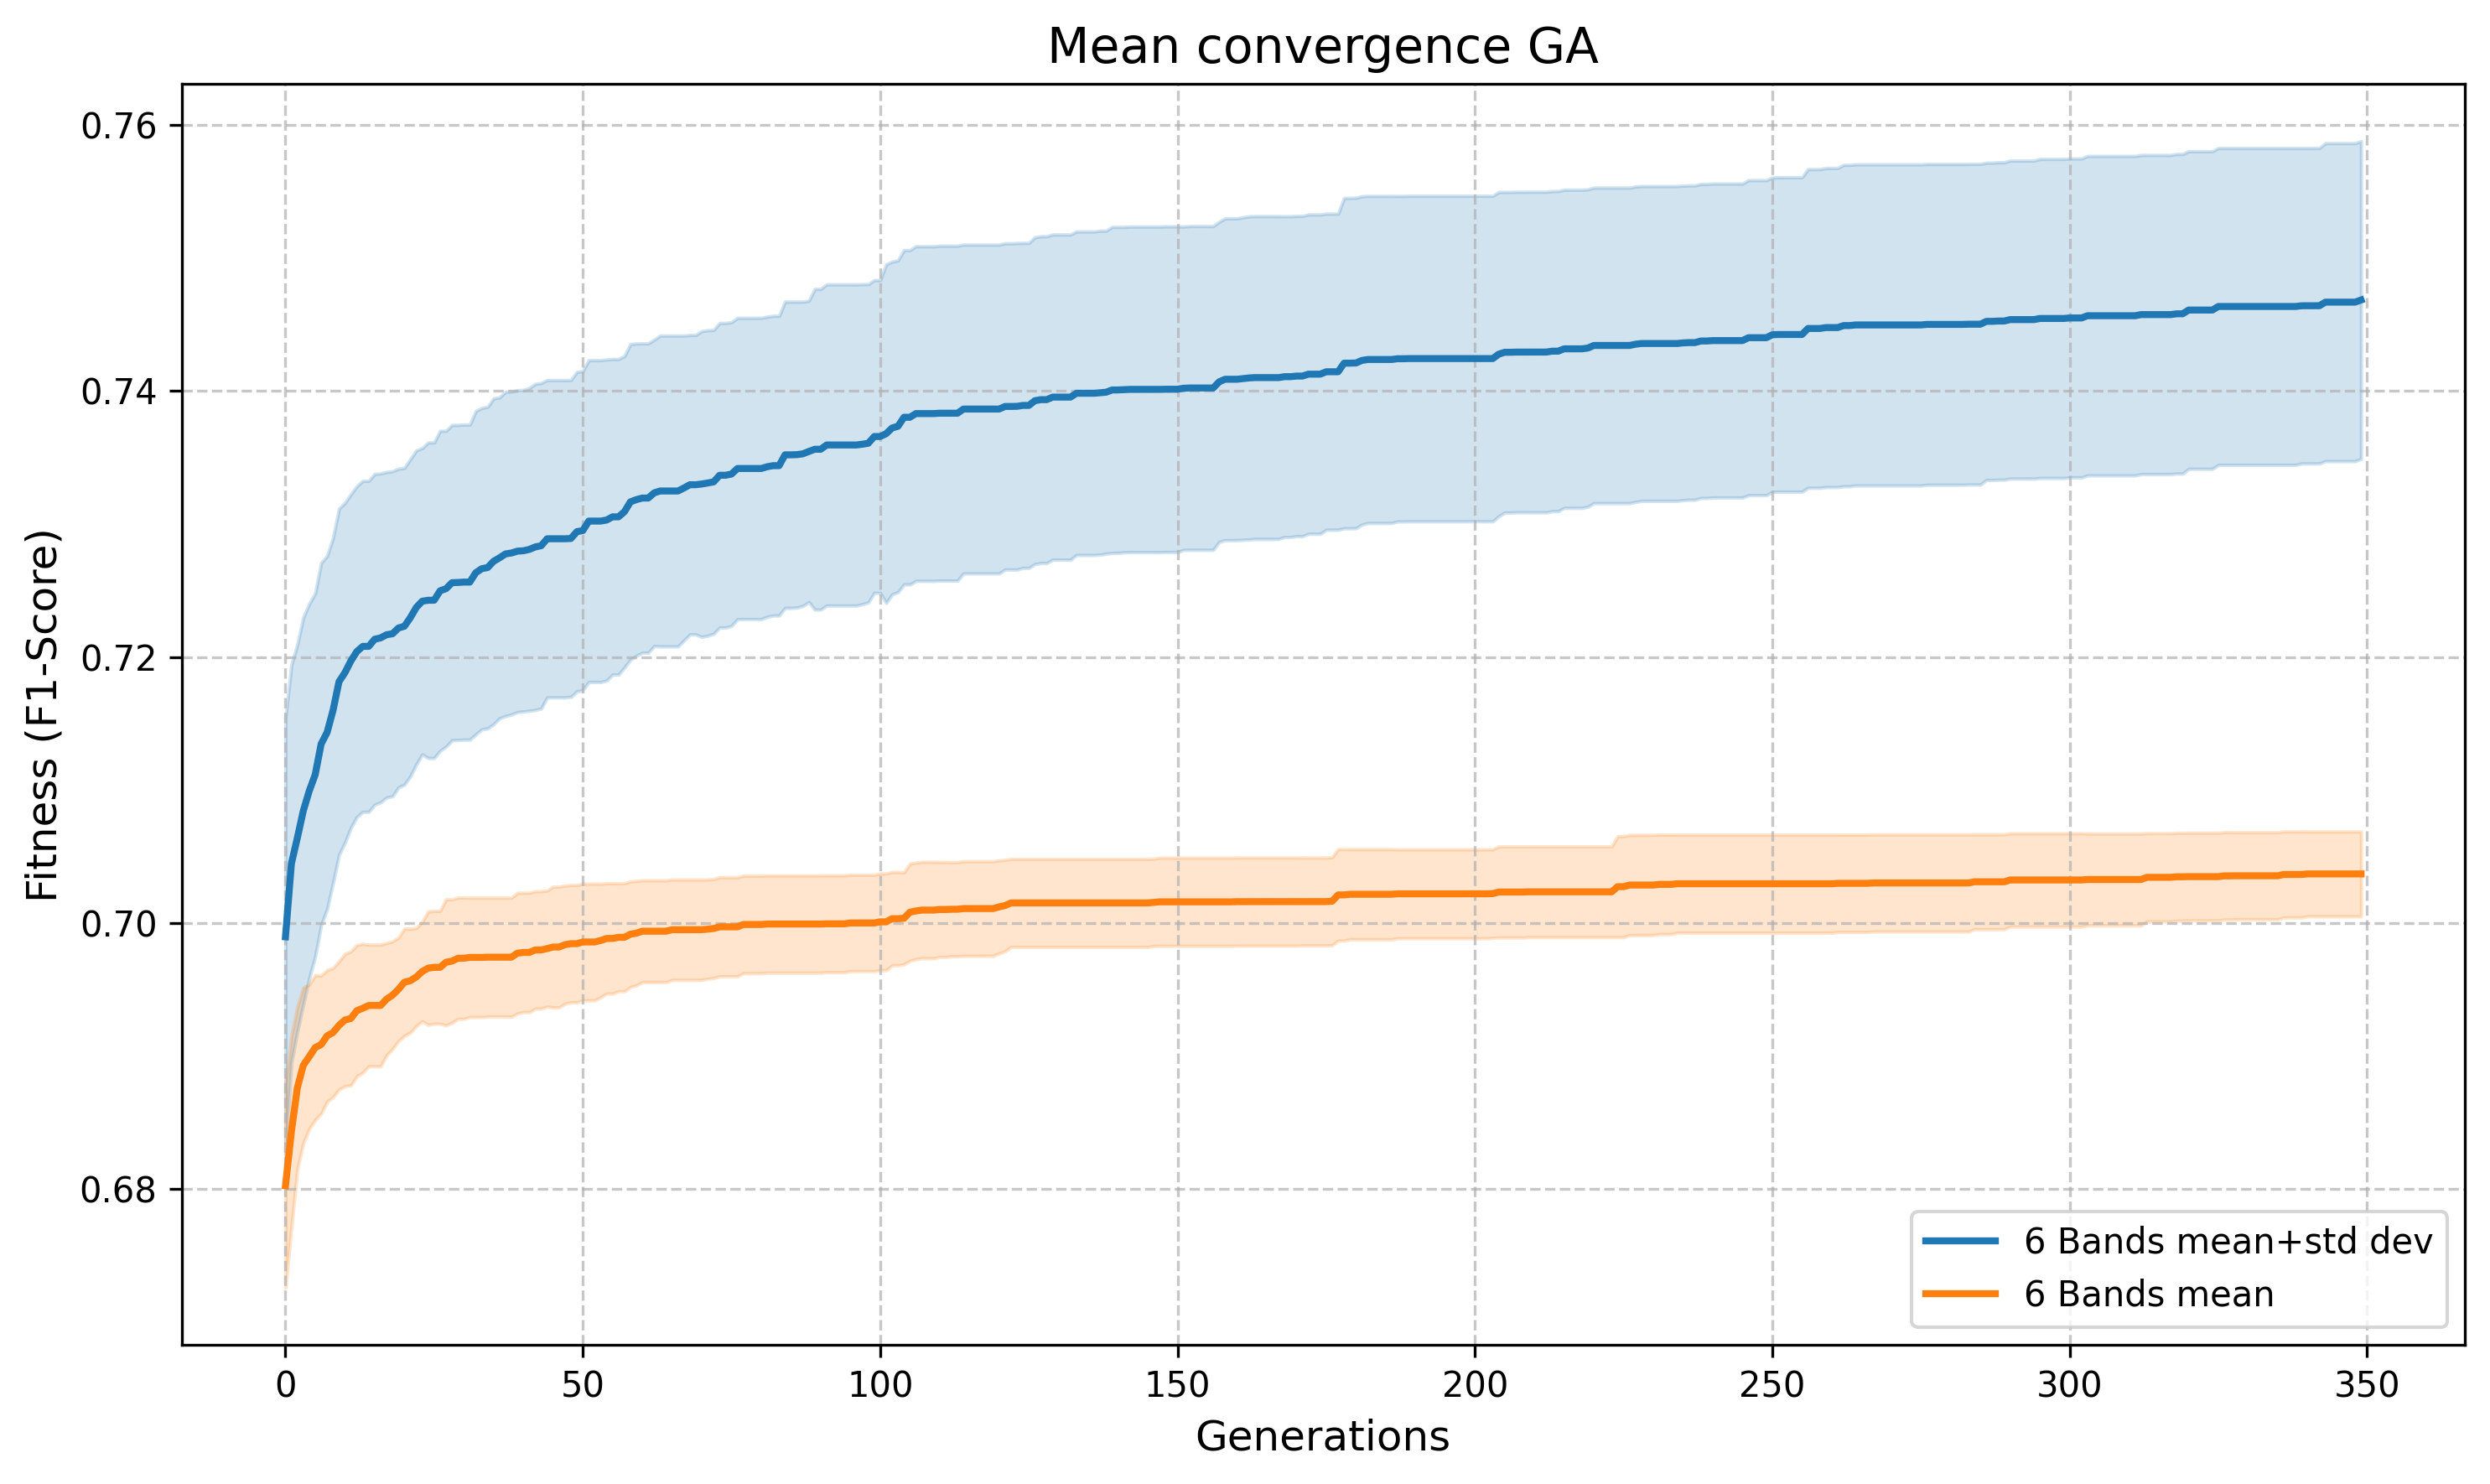
\includegraphics[width=8.2cm]{Imagenes/mean_convergence_6b.png}}
\hfill
%\end{adjustwidth}
%\caption{Convergence history of the Genetic Algorithm over 30 independent runs. (\textbf{a}) 3 bands optimization. (\textbf{b}) 5 bands optimization. (\textbf{c}) 6 bands optimization.\label{fig:4}}
\caption{Media de convergencia de las ejecuciones del algoritmo genetico durante 30 ejecuciones independientes para los escenarios: (\textbf{a}) 3 Bandas; (\textbf{b}) 5 Bandas; y (\textbf{c}) 6 Bandas.\label{fig:ga_convergence}}
\end{figure} 

\subsection{Análisis Comparativo del Rendimiento: GA y PSO}
Tras validar la construcción del vector, el segundo análisis se enfocó en contrastar las capacidades de optimización global del Algoritmo Genético frente a la Optimización por Enjambre de Partículas. La distribución estadística de los valores F1-Score obtenidos tras 30 ejecuciones independientes se resume mediante diagramas de caja en la Figura \ref{fig:boxplot_ga_pso}.
\begin{figure}[H]
\centering
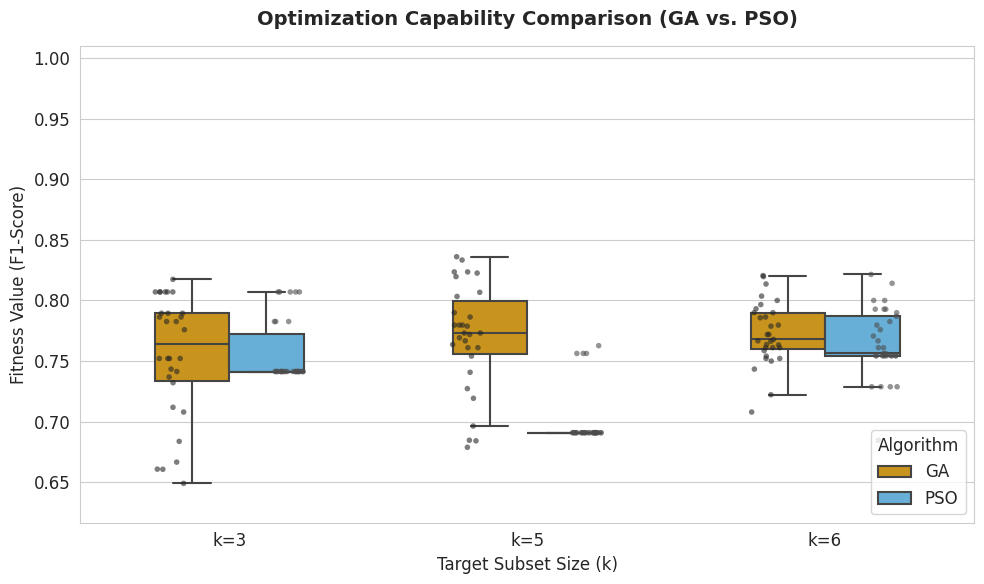
\includegraphics[width=12.0 cm]{Imagenes/boxplot_comparison_mean_std.png}
\caption{Diagrama de cajas: comparación de GA vs. PSO con características ($\mu+\sigma$).}
\label{fig:boxplot_ga_pso}
\end{figure}   
\unskip
\hfill \break

\begin{figure}[H]
\centering
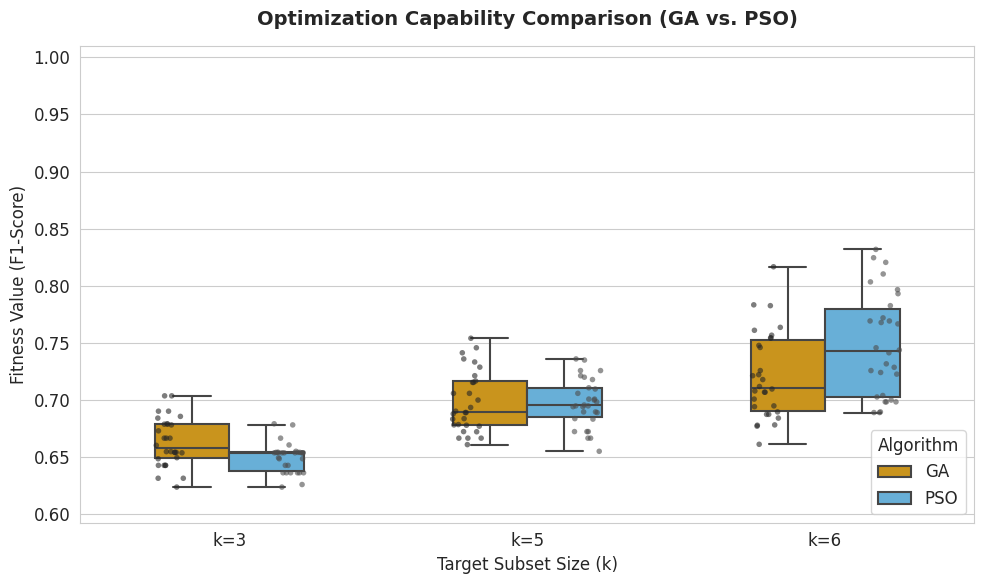
\includegraphics[width=12.0 cm]{Imagenes/boxplot_comparison_mean.png}
\caption{Diagrama de cajas: comparación de GA vs. PSO únicamente con media ($\mu$).}
\label{fig:boxplot_ga_pso_mean}
\end{figure}   
\unskip

El análisis comparativo revela que ambas metaheurísticas son altamente competentes para la selección de bandas hiperespectrales, aunque presentan sutiles diferencias en su comportamiento. El GA demostró una consistencia general ligeramente superior, exhibiendo una mediana de F1-Score más alta y rangos intercuartílicos más estrechos para los subconjuntos de 5 y 6 bandas. Esta menor dispersión indica una mayor estabilidad algorítmica y reproducibilidad en sus resultados.

Por otro lado, el algoritmo PSO mostró una ligera ventaja competitiva en el escenario más restrictivo (3 bandas). Más importante aún, el PSO fue el algoritmo capaz de encontrar el óptimo absoluto global de todo el estudio: un F1-Score máximo de 0.836 utilizando la configuración de 5 bandas combinadas. Este hallazgo subraya la excelente capacidad de explotación local que otorgan los Coeficientes de Aceleración Variables en el Tiempo (TVAC) implementados en el PSO.

En conclusión, los resultados validan que es posible reducir drásticamente la dimensionalidad de los datos hiperespectrales (pasando de cientos de bandas a un conjunto óptimo de cinco) sin sacrificar la precisión diagnóstica para la detección de Aspergillus flavus, sentando un precedente viable para la implementación de futuros sistemas de inspección agrícola.